%
% xtal formulas
% @author Tobias Weber <tweber@ill.fr>
% @date 13-jul-2018
% @license see 'LICENSE' file
%

\chapter{Crystal and Instrument Coordinate Systems}
\label{ch:xtal}

In this chapter we review the theory for conversion between crystal coordinates and scattering angles 
at the triple-axis instrument. Section \ref{sec:xtalcoords} introduces crystal coordinates and the so-called 
$UB$ matrix formalism, section \ref{sec:tasangles} calculates the corresponding TAS angles. 
The formalisms \cite{Lumsden2005} reviewed here are ubiquitous in neutron science, they are not only used 
in the control programs of triple-axis instruments, among them \textit{NOMAD} \cite{web_NOMAD} 
or \textit{NICOS} \cite{web_NICOS}, but are also employed in virtual instrument simulators like \textit{vTAS} \cite{vTAS2013} or 
\textit{McStas} \cite{McStas2020}, as well as in data analysis software like \textit{Mantid} \cite{Arnold2014}.

Note that this chapter has already been published in the manual of the software from Ref. \cite{Takin2021},
as well as in my (physics) PhD thesis \cite[pp. 139-143]{PhDWeber},
where the latter featured an earlier version of the same text, figures, and derivations.
Originally, these formulas were re-derived with the aid of the source
code of \textit{McStas'} \textit{templateTAS} virtual instrument \cite{web_mcstas_templateTAS, McStas2020}.


% ------------------------------------------------------------------------------------------------------------------------------------
\section{Fractional crystal coordinates \label{sec:xtalcoords}}

We begin by presenting the so-called $UB$ matrix formalism to convert between relative lattice units 
of a crystal and laboratory coordinates used in instrument space. This method has been described in 
Ref. \cite{Lumsden2005}. The derivation of the transformation matrices, $A$ and $B$, describing fractional
crystal coordinates, can be found in \cite{wiki_fractional}, which we follow here.

\subsection{$A$ and $B$ matrices}
\paragraph{Real-space crystal lattice}
The unit cell of the crystal is spanned by its three basis vectors $\left| a \right>$, $\left| b \right>$, and $\left| c \right>$, 
which -- in general -- are not perpendicular to one another, but instead enclose angles of $\alpha$, $\beta$, 
and $\gamma$, respectively, as shown in Fig. \ref{fig:cell}. 
To calculate the crystallographic $A$ matrix which transforms non-orthogonal crystal to orthogonal lab units, 
we first need to reduce the number of parameters.
The respective relations between the three basis vectors and their angles can be directly obtained via
their scalar products, where we follow the derivation in Ref. \cite{wiki_fractional}:

\vspace{\abovedisplayskip}
\begin{minipage}{0.317\textwidth}
	\begin{equation} \left< a | b \right > \ =\  ab \cos \gamma, \label{eq:ab} \end{equation}
\end{minipage}
\begin{minipage}{0.317\textwidth}
	\begin{equation} \left< a | c \right > \ =\  ac \cos \beta, \label{eq:ac} \end{equation}
\end{minipage}
\begin{minipage}{0.317\textwidth}
	\begin{equation} \left< b | c \right > \ =\  bc \cos \alpha. \label{eq:bc} \end{equation}
\end{minipage}
\vspace{\belowdisplayskip}

\begin{figure}
	\centering
	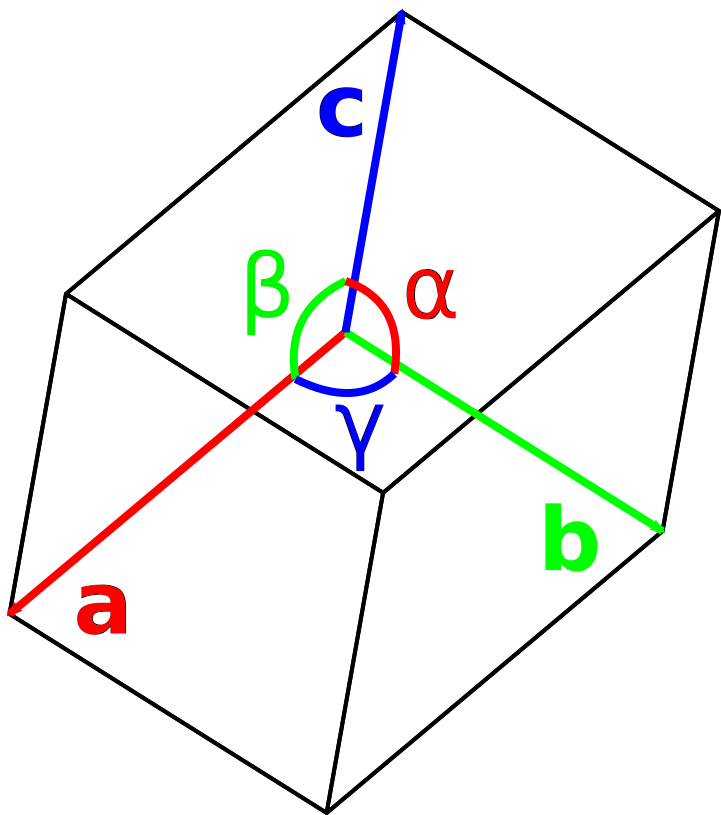
\includegraphics[width = 0.2 \textwidth]{figures/cell}
	\caption[Crystal unit cell.]{
		The unit cell of a crystal is given by its coordinate vectors $a$, $b$, and $c$ 
		as well as their angles $\alpha$, $\beta$, and $\gamma$.
		Figure drawn after the figure in Ref. \cite{wiki_fractional}.}
	\label{fig:cell}
\end{figure}


%\subsection*{Basis vectors}

The next goal is to explicitly write the components of the vectors $\left| a \right>$, $\left| b \right>$, and $\left| c \right>$ 
in terms of their lengths $a = \sqrt{\left< a | a \right>}$, $b = \sqrt{\left< b | b \right>}$, $c = \sqrt{\left< c | c \right>}$,
and the three angles.
To that end, we first choose -- without loss of generality -- $\left| a \right>$ along the $x$ axis, $\left| b \right>$ in the 
$xy$ plane, and $\left| c \right>$ in general:
\begin{equation} 
	\boxed{ \left| a \right> \ =\  \left( \begin{array}{c} a_1 = a \\ 0 \\ 0 \end{array} \right), }
	\hspace{0.5cm} \left| b \right> \ =\  \left( \begin{array}{c} b_1 \\ b_2 \\ 0 \end{array} \right),
	\hspace{0.5cm} \left| c \right> \ =\  \left( \begin{array}{c} c_1 \\ c_2 \\ c_3 \end{array} \right).
\end{equation}


Inserting $\left| a \right>$ and $\left| b \right>$ into Eq. \ref{eq:ab} gives the first component
of the $\left| b \right>$ vector:
\begin{equation} \left< a | b \right > \ =\  a_1 b_1 \ =\  ab \cos \gamma
\hspace{0.5cm} \Rightarrow \hspace{0.5cm} b_1 \ =\  b \cos \gamma. \end{equation}


Using the cross product between $\left| a \right>$ and $\left| b \right>$, we get the second component of $\left| b \right>$:
\begin{equation} 
	\left\Vert \left| a \right> \times \left| b \right> \right\Vert \ =\ 
	\left\Vert \left( \begin{array}{c} 0 \\ 0 \\ a_1 b_2 \end{array} \right) \right\Vert \ =\ 
	ab \sin \gamma \label{eq:crossab}
	\hspace{0.5cm} \Rightarrow \hspace{0.5cm} b_2 \ =\  b \sin \gamma.
\end{equation}

The vector $\left| b \right>$ is now complete:
\begin{equation} 
\boxed{ \left| b \right> \ =\  \left( \begin{array}{c} b \cos \gamma \\ b \sin \gamma \\ 0 \end{array} \right). } 
\label{eq:bvec} 
\end{equation}


Inserting $\left| a \right>$ and $\left| c \right>$ into Eq. \ref{eq:ac} gives the first component of $\left| c \right>$:
\begin{equation} \left< a | c \right > \ =\  a_1 c_1 \ =\  ac \cos \beta
\hspace{0.5cm} \Rightarrow \hspace{0.5cm} c_1 \ =\  c \cos \beta.
\end{equation}



Inserting $\left| b \right>$ and $\left| c \right>$ into Eq. \ref{eq:bc} yields the second component of $\left| c \right>$:
\begin{equation} \left< b | c \right > \ =\  b_1 c_1 + b_2 c_2 \ =\  bc \cos \alpha, \end{equation}
\begin{equation} b \cos \gamma \cdot c \cos \beta + b \sin \gamma \cdot c_2 \ =\  bc \cos \alpha
	\hspace{0.5cm} \Rightarrow \hspace{0.5cm}
	c_2 \ =\  \frac{c \cos \alpha - c \cos \gamma \cos \beta}{\sin \gamma}. \end{equation}



The last component, $c_3$, can be obtained from the vector length normalisation, $ \left< c | c \right> = c^2 $:
\begin{equation} \left< c | c \right > \ =\  c_1^2 + c_2^2 + c_3^2 \ =\  c^2, \end{equation}
\begin{equation} c_3^2 \ =\  c^2 - c_1^2 - c_2^2
	\hspace{0.5cm} \Rightarrow \hspace{0.5cm}
	c_3^2 \ =\  c^2 \left[1 - \cos^2 \beta - \left(\frac{\cos \alpha - \cos \gamma \cos \beta}{\sin \gamma} \right)^2 \right].
\end{equation}

The full vector $\left| c \right>$ is now reads:
\begin{equation} \boxed{ \left| c \right> \ =\  \left( \begin{array}{c}
	c \cdot \cos \beta \\
	c \cdot \frac{\cos \alpha - \cos \gamma \cos \beta}{\sin \gamma} \\
	c \cdot \sqrt{ \sin^2 \beta - \left(\frac{\cos \alpha - \cos \gamma \cos \beta}{\sin \gamma} \right)^2 }
\end{array} \right). } \end{equation}



The crystallographic $A$ matrix, which transforms real-space fractional to lab coordinates (\AA) \cite{Lumsden2005},
is formed with the basis vectors in its columns \cite[p. 631]{Arens2015}:
\begin{equation}
	A \ =\  \left(
		\begin{array}{ccc}
			\left| a \right> & \left| b \right> & \left| c \right>
		\end{array}
	\right).
\end{equation}
Explicitly written out using the basis vectors, the matrix reads \cite{wiki_fractional}:
\begin{equation}
	A \ =\  \left(
		\begin{array}{ccc}
			\begin{array}{c} a \\ 0 \\ 0 \end{array}
			& 
			\begin{array}{c} b \cos \gamma \\ b \sin \gamma \\ 0 \end{array} 
			& 
			\begin{array}{c}
				c \cdot \cos \beta \\
				c \cdot \frac{\cos \alpha - \cos \gamma \cos \beta}{\sin \gamma} \\
				c \cdot \sqrt{ \sin^2 \beta - \left(\frac{\cos \alpha - \cos \gamma \cos \beta}{\sin \gamma} \right)^2 }
			\end{array}
		\end{array}
	\right).
\end{equation}


\paragraph{Reciprocal-space crystal lattice}
For calculations in solid-state physics and neutron scattering, one does not normally use
the real-space crystal lattice, but instead thinks in term of the so-called reciprocal-space
lattice \cite[pp. 11-15]{Shirane2002}.
Reciprocal space is constructed in a way to facilitate calculations with momenta on a periodic lattice,
for that reason it is also sometimes called momentum or Fourier space.
A comparison of the same Bragg scattering in real vs. reciprocal space is shown in Fig. \ref{fig:braggscattering_recip}.
It is obvious that the reciprocal view greatly simplifies the image: Bragg scattering on what is a set of parallel
crystal planes in real space in panel (a) becomes a single point in reciprocal space \cite[p. 66]{Gross2012},
the so-called Bragg peak $\left| G \right>$ in panel (c). The reciprocal vector $\left| G \right>$ is
perpendicular to the original crystal planes and its length is related to their distance $d$ by
$\left\Vert G \right\Vert = 2\pi/d$ \cite[p. 66]{Gross2012}. Panel (c) also shows how the lattice vector
together with the neutron beam directions forms the so-called scattering triangle, which is 
ubiquitous in visualisations of neutron scattering geometry \cite[pp. 14-15]{Shirane2002} and which will be 
discussed in the next section.
\begin{figure}[htb]
	\centering
	\includegraphics[width=1\textwidth]{figures/bragg_recip}
	\caption[Real and reciprocal lattice scattering.]{
		(a) Bragg scattering on crystal planes having a spacing $d$, viewed from real space.
			Figure drawn after Ref. \cite[p. 68, Fig. 2.7]{Gross2012}.
		(b) A view mixing real and reciprocal space. The reciprocal lattice vector, $\underline{G}$,
			is perpendicular to the real space crystal planes.
		(c) Bragg scattering viewed from reciprocal space. The direction of the incoming and outgoing
			neutron beams define wavevectors $\underline{k}_i$ and $\underline{k}_f$.
			Such a representation is called a scattering diagram or scattering triangle
			\cite[p. 14, Fig. 1.5]{Shirane2002}.}
	\label{fig:braggscattering_recip}
\end{figure}

From the construction of reciprocal space, it can be shown that the basis vectors of reciprocal space
are mutually perpendicular to the corresponding real space basis vectors \cite[p. 60]{Gross2012}.
This directly leads to the so-called $B$ matrix, which transforms reciprocal-space relative lattice units (rlu)
to lab coordinates (1/\AA) \cite{Lumsden2005}, is \cite[p. 60]{Gross2012}:
\begin{equation} B \ =\  2 \pi A^{-t}, \end{equation}
where $-t$ denotes the transposed inverse.
We can now also determine the metric tensor \cite[pp. 807-809]{Arens2015} corresponding to the coordinate
system defined by the $B$ transformation matrix, it reads \cite[p. 808]{Arens2015}:
\begin{equation}
	\left(g_{ij}\right) \ =\  \left<\underline{b}_i | \underline{b}_j \right> \ =\  B^T B,
\end{equation}
where the reciprocal basis vectors $\left| \underline{b}_i \right>$ form the columns of $B$ \cite[p. 631]{Arens2015}.

A rigorous introduction into the reciprocal crystal lattice can be found in the book by Gross
and Marx \cite[pp. 58 - 67]{Gross2012}.


\subsection{Example: lengths and angles in the reciprocal lattice}
Having a metric makes it straightforward to calculate lengths and angles.
The length of a reciprocal lattice vector $\left| G \right>$ seen from the lab system is 
(in 1/\AA{} units) \cite[p. 808]{Arens2015}:
\begin{equation}
	\left\Vert \left< G | G \right> \right\Vert \ =\  \sqrt{\left< G | G \right>}
		\ =\  \sqrt{G_i G^i} \ =\  \sqrt{g_{ij} G^i G^j}.
\end{equation}
The angle $\theta$ between two Bragg peaks $\left| G \right>$ and $\left| H \right>$ 
is given by their dot product \cite[p. 808]{Arens2015}:
\begin{equation}
	\frac{\left< G | H \right>}{\left\Vert \left< G | G \right> \right\Vert
		\cdot \left\Vert \left< H | H \right> \right\Vert} \ =\
	\frac{g_{ij} G^i H^j }{\sqrt{g_{ij} G^i G^j} \sqrt{g_{ij} H^i H^j}} \ =\  \cos \theta.
\end{equation}

Please note that if an index appears twice, both as subscript as well as a superscript, 
a summation over it is implied, see Ref. \cite{wiki_summation}.


\subsection{$U$ matrix}
The $B$ matrix alone yields the transformation from the non-orthogonal and reciprocal crystal 
coordinate system into the orthogonal lab units \cite{Lumsden2005}.
However, it does not yet take into account the actual rotation of the crystal so that a specific plane, 
the so-called scattering plane, can be accessed by the two-dimensional movements of the instrument. 
Such a rotation is performed by the $U$ matrix, whose rows contain two vectors inside the desired 
scattering plane and the plane normal \cite{Lumsden2005}.
These basis vectors are usually chosen along two orientation Bragg reflections \cite[pp. 87-88]{Shirane2002}
and are expressed in the orthogonal lab system, i.e. they are pre-multiplied by $B$.
For $U$ to be a rotation matrix, the basis vectors are normalised using, for instance, the
Gram-Schmidt algorithm \cite[p. 744]{Arens2015} \cite[pp. 269-270]{Arfken2013} or 
QR decomposition \cite[pp. 269-272]{Scarpino2011}.

In summary, a coordinate point $\left|Q_{\mathrm{rlu}}\right>$, which is given in relative lattice 
units of the reciprocal crystal, 
is transformed by the $B$ matrix into the orthogonal lab units used at the instrument \cite{Lumsden2005}.
It is then rotated by the $U$ matrix to account for the actual crystal orientation \cite{Lumsden2005}:
\begin{equation}
	\left|Q_{\mathrm{lab}}\right> \ =\  U \cdot B \cdot \left|Q_{\mathrm{rlu}}\right>.
\end{equation}
In the rest of this work we will not use the $U$ matrix explicitly, though, but instead directly work 
with its basis vectors. This is just a formality, though, the mathematics are the same.

% ------------------------------------------------------------------------------------------------------------------------------------




% ------------------------------------------------------------------------------------------------------------------------------------
\section{Scattering triangle and TAS angles \label{sec:tasangles}}

With the metric tensor \cite[pp. 807-809]{Arens2015} of the crystal coordinate system, we can now calculate the scattering angles
$2 \theta_M$, $2 \theta_S$, and $2 \theta_A$ from the monochromator, sample and analyser, respectively. 
The derivation of basic scattering geometries in triple-axis spectrometers can be found in \cite[Ch. 1.3]{Shirane2002},
which we follow here. 
The explicit calculation of the TAS angles based on the $UB$ formalism was originally presented in Ref. \cite{Lumsden2005}.

For the monochromator and analyser, the crystal angles $\theta_M$ and $\theta_A$ are coupled to 
their scattering angles, they are simply half their value, because the Bragg condition of Eq. \ref{eq:bragg}
always has to be fulfilled.
The crystal rotation for the sample is not necessarily half its scattering angle, $\Theta_S \ne 2\theta_S/2$, 
though, because the instrument can be freely positioned at any point of reciprocal crystal space.

The monochromator and analyser scattering angles follow directly from Bragg's equation 
\cite[p. 68]{Gross2012} \cite[p. 13]{Shirane2002}:

\begin{minipage}{0.45\textwidth}
	\centering
	\begin{equation} 2 d_{M}\sin \theta_{M} \ =\  n \lambda_{i}, \end{equation}
	\begin{equation} 2 k_{i} \sin \theta_{M} \ =\  2 \pi n / d_{M}, \end{equation}
	\begin{equation} \boxed{ \theta_{M} \ =\  \arcsin \left( \frac{\pi n}{d_{M} \cdot k_{i}} \right). } \end{equation}
\end{minipage}
\begin{minipage}{0.45\textwidth}
	\centering
	\begin{equation} 2 d_{A}\sin \theta_{A} \ =\  n \lambda_{f}, \end{equation}
	\begin{equation} 2 k_{f} \sin \theta_{A} \ =\  2 \pi n / d_{A}, \end{equation}
	\begin{equation} \boxed{ \theta_{A} \ =\  \arcsin \left( \frac{\pi n}{d_{A} \cdot k_{f}} \right). } \end{equation}
\end{minipage}

%\vspace{0.5cm}

To determine the sample scattering angle $2 \theta_S$, we use the so-called scattering triangle, see 
Fig. \ref{fig:scattering_triangle}, whose connection to the neutron beam direction has already 
been established in the previous section.
The scattering triangle can be directly determined by the angles the instrument is positioned at \cite[pp. 14-15]{Shirane2002}: 
For that, we have a look at the incoming and final neutron wavevectors $\left| k_i \right>$ and $\left| k_f \right>$, 
whose directions (but not lengths!) correspond directly to the neutron paths before and after the sample, 
respectively, as shown on the left-hand side of Fig. \ref{fig:scattering_triangle}. We can rearrange them so 
that their tips meet, as depicted on the right-hand side of Fig. \ref{fig:scattering_triangle}, where the 
scattering triangle is formed by $\left| k_i \right>$ and $\left| k_f \right>$ together with the
scattering vector $\left| Q \right> = \left| k_i \right> - \left| k_f \right>$ \cite[p. 14]{Shirane2002}.
Here, the two wavevectors enclose the scattering angle $2 \theta_S$.

\begin{figure}
	\begin{center}
		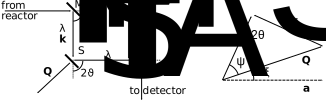
\includegraphics[width = 0.75 \textwidth]{figures/tas_triangle}
	\end{center}
	\caption[TAS layout and scattering triangle.]{
		Triple-axis layout (left) and corresponding scattering triangle (right).
		Figures inspired by Ref. \cite[p. 72, Fig. 3.8]{Shirane2002} and \cite[p. 15, Fig. 1.6]{Shirane2002}, respectively.
		\label{fig:scattering_triangle}}
\end{figure}

We can calculate $2 \theta_S$ via the cosine theorem \cite[pp. 694-695]{Arens2015}, i.e.
by forming the scalar product of $\left| Q \right>$ with itself \cite[p. 11]{Shirane2002}:
\begin{equation} 
	\left| Q \right> \ =\  \left| k_i \right> - \left| k_f \right>,
\end{equation}
\begin{equation} 
	\left< Q | Q \right> \ =\  \left( \left< k_i \right| - \left< k_f \right| \right) \cdot \left( \left| k_i \right> - \left| k_f \right> \right)
	\ =\  \left< k_i | k_i \right> + \left< k_f | k_f \right> - 2 \left< k_i | k_f \right>,
\end{equation}
\begin{equation} 
	Q^2 \ =\  k_i^2 + k_f^2 - 2 k_i k_f \cos \left( 2 \theta_S \right),
\end{equation}
\begin{equation}
	\boxed{ 2 \theta_S \ =\  \sigma_s \cdot \arccos \left( \frac{k_i^2 + k_f^2 - Q^2}{2 k_i k_f} \right). }
\end{equation}

As we could scatter in either clockwise or counter-clockwise direction, $2 \theta_S$ can be positive or negative.
The sign of $2 \theta_S$ is given by the sample scattering sense $\sigma_s = \pm 1$.


%\vspace{0.5cm}


The final and most complicated angle to determine is the sample rotation $\Theta_S$.
It is given by the angle of the incoming wavevector $\left| k_i \right>$ to an (arbitrary) direction 
$\left| a \right>$ which is known from sample orientation, this is usually a Bragg peak \cite[p. 87]{Shirane2002}.
If we were to explicitly use the $U$ matrix here, this vector would be one of its rows.
The situation is shown in the right panel of Fig. \ref{fig:scattering_triangle}.
We split $\Theta_S$ into the angle $\psi$ between $\left| k_i \right>$ and $\left| Q \right>$ 
and the angle $\xi$ between $\left| Q \right>$ and $\left| a \right>$:
\begin{equation} \boxed{ \Theta_S \ =\  180^{\circ} - \left( \psi + \xi \right).} \end{equation}


%\vspace{0.5cm}


The angle $\psi$ between $\left| k_i \right>$ and $\left| Q \right>$ is determined from the scattering triangle, as before:
\begin{equation}
	\left| k_f \right> \ =\  \left| k_i \right> - \left| Q \right>,
\end{equation}
\begin{equation} 
	\left< k_f | k_f \right> \ =\  \left( \left< k_i \right| - \left< Q \right| \right) \cdot \left( \left| k_i \right> - \left| Q \right> \right)
	\ =\  \left< k_i | k_i \right> + \left< Q | Q \right> - 2 \left< k_i | Q \right>,
\end{equation}
\begin{equation}
	k_f^2 \ =\  k_i^2 + Q^2 - 2 k_i Q \cos \psi,
\end{equation}
\begin{equation}
	\boxed{ \psi \ =\  \sigma_s \cdot \arccos \left( \frac{k_i^2 + Q^2 - k_f^2}{2 k_i Q} \right).}
\end{equation}


%\vspace{0.5cm}


The angle $\xi$ between $\left| Q \right>$ and orientation vector $\left| a \right>$ is also determined 
from the properties of the scalar product.
Here we have to use its covariant form via the metric tensor, $g_{ij}$, \cite[p. 808]{Arens2015},
because $\left| a \right>$ is a coordinate in crystal space naming a Bragg reflection,
while $\left| Q \right>$ lives, as before, in instrument space.
\begin{equation} 
	\boxed{ \xi \ =\  
\sigma_{\mathrm{side}} \cdot \arccos \left( \frac{ \left< Q | a \right> }{ \sqrt{\left< Q | Q \right>} \sqrt{\left< a | a \right>} } \right) \ =\  
\sigma_{\mathrm{side}} \cdot \arccos \left( \frac{ Q^i g_{ij} a^j }{ \sqrt{Q^i g_{ij} Q^j} \sqrt{a^i g_{ij} a^j} } \right).}
\label{eq:xi}
\end{equation}

The sign, $\sigma_{\mathrm{side}}$, of $\xi$ depends on which side of the orientation vector 
$\left| a \right>$ the scattering vector $\left| Q \right>$ is located. 
The sign can be found by calculating the (covariant) cross product of $\left| a \right>$ and 
$\left| Q \right>$ to give an out-of-plane vector $\left| x \right>$ which can be compared with 
the given scattering plane up vector.
The covariant cross-product is calculated as \cite[p. 815]{Arens2015}:
\begin{equation}
	x^l \ =\  g^{li} \epsilon_{ijk} a^j Q^k,
\end{equation}
where $\epsilon_{ijk}$ is the general Levi-Civita symbol formed from the determinant of the 
basis vectors $\left| \underline{b}_i \right>$, see Ref. \cite[p. 815]{Arens2015}:
\begin{equation}
	\epsilon_{ijk} \ =\  \left|
		\begin{array}{ccc} \left| 
			\underline{b}_i \right> & \left| \underline{b}_j \right> & \left| \underline{b}_k \right>
		\end{array} \right|.
\end{equation}



\paragraph*{Special case}
For cubic crystals with $\alpha = \beta = \gamma = 90^{\circ}$ and the lattice constants all equal, 
$a = b = c$, the metric tensor is diagonal, $g_{ij} = \delta_{ij} \cdot \left( 2\pi / a \right)^2$.
With that Eq. \ref{eq:xi} simplifies to:
\begin{equation}
	\xi \ =\  \sigma_{\mathrm{side}} \cdot \arccos \left( \frac{ Q_i a^i }{ \sqrt{Q_i Q^i} \sqrt{a_i a^i} } \right).
\end{equation}
% ------------------------------------------------------------------------------------------------------------------------------------


\section{Summary}
This chapter introduced some important concepts from solid-state physics and crystallography that are essential
for an understanding of the basic coordinate system transformations from the generally non-orthogonal (real or 
reciprocal) crystal coordinates to the orthonormal lab coordinates used at the instrument.
In practice, it is the crystal coordinates that are entered into the instrument control software by
the user, not the raw instrument angles. A pathfinding system for triple-axis spectrometers thus has to know both.
Internally, it will be more convenient for the software to use instrument-related coordinates, as we will see in 
the following chapters, but the input and output will be in crystal coordinates.

Having established all the necessary physical foundations, the next chapter will proceed to do the same for the 
essential concepts in computer science before putting everything together in a pathfinding algorithm.
